%%%%%%%%%%%%%%%%%%%%%%%%%%%%%%%%
\section{Driving Profile and Non-Propulsion Power Modeling, Estimation, and Runtime Optimization} \label{sec:driving_profile}
%%%%%%%%%%%%%%%%%%%%%%%%%%%%%%%%

%%%%%%%%%%%%%%%%%%%%%%%%%%%%%%%%
\subsection{Introduction and Background}

%Electric Vehicle (EV) as a multi-domain Cyber-Physical System (CPS) consists of two major systems of electric motor and auxiliary system that are the main contributors to the power consumption~\cite{AF_1,AF_2,AF_3,AF_4}.
%
%\textbf{Electric motor} is the main system that generates enough force to propel the vehicle at a desired speed and acceleration. The electric motor consumes the energy stored in a storage such as a lithium-ion battery for generating the driving power and force. The electric motor can also behave as a generator; hence, the electric motor can generate electric power while generating driving power and force in the opposite direction. This regenerative braking system helps the EVs achieve higher energy efficiency and extended driving range~\cite{AF_5,AF_6,AF_7}.
%
%\textbf{Propulsion power} generated or consumed by the electric motor significantly influences the stored battery energy, the EV driving range, and the battery lifetime~\cite{AF_8,AF_9,AF_10}. Hence, modeling, estimation, and optimization of the propulsion power is a major solution to extending the driving range and battery lifetime.

One of the main factors that influence the propulsion power is the driving behavior of the EV. The driving behavior can be modeled by the values of the driving speed, acceleration, and deceleration at each time instance of the driving route as the \textbf{driving profile}. For instance, as shown in Fig.~\ref{AF_image1}, the driving speed influences the electric motor power consumption considering the gravitational, aerodynamic, rolling resistance forces~\cite{AF_6}. 

\begin{figure}
\centering
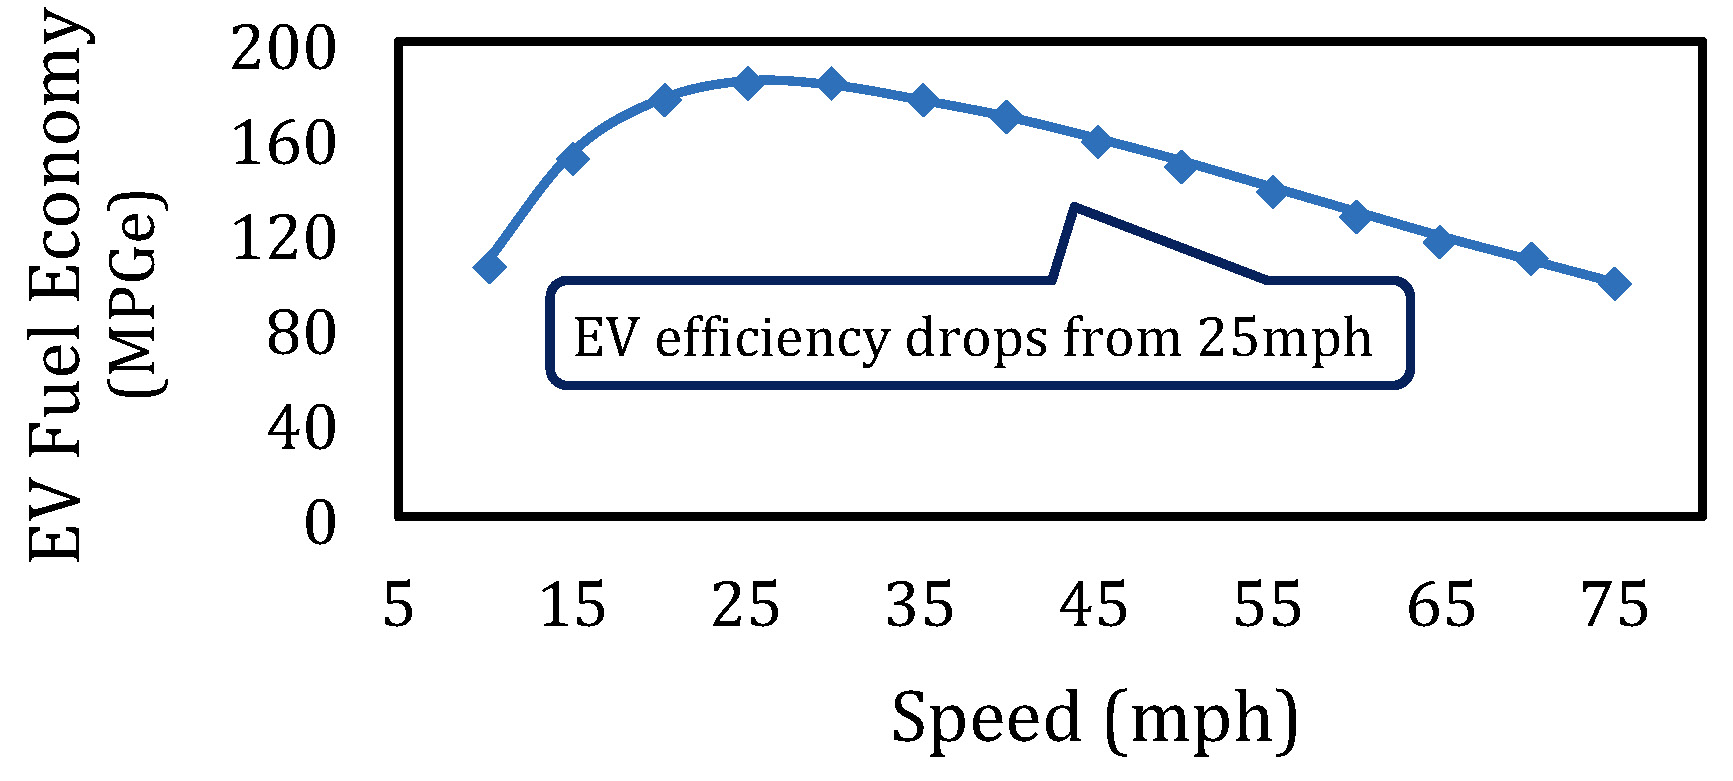
\includegraphics[width=0.7\hsize]{Figures/Al_Faruque/AF_figure1.jpeg}
\caption{EV fuel economy for different driving speeds~\cite{AF_11,AF_10}.}
\label{AF_image1}
\end{figure}      

Therefore, modeling and estimation of the driving profile not only helps in estimating the driving habits of the drivers, but also enables the designers and engineers in modeling, estimation, and later optimization of the propulsion power in the EV. On the other hand, adjusting and optimizing the driving profile itself is another effective approach to extending the driving range and battery lifetime~\cite{AF_11}. 

Auxiliary systems in the EV are the other major systems which influence its power consumption. \textbf{Non-propulsion} power requested by the auxiliary systems mostly depend on the functionality and objective of the system regardless of the driving behavior and profile. For instance, HVAC system as an auxiliary system is responsible to maintain the cabin temperature in a comfort thermal range for the passengers~\cite{AF_13,AF_14,AF_15,AF_16}.

\begin{figure}
\centering
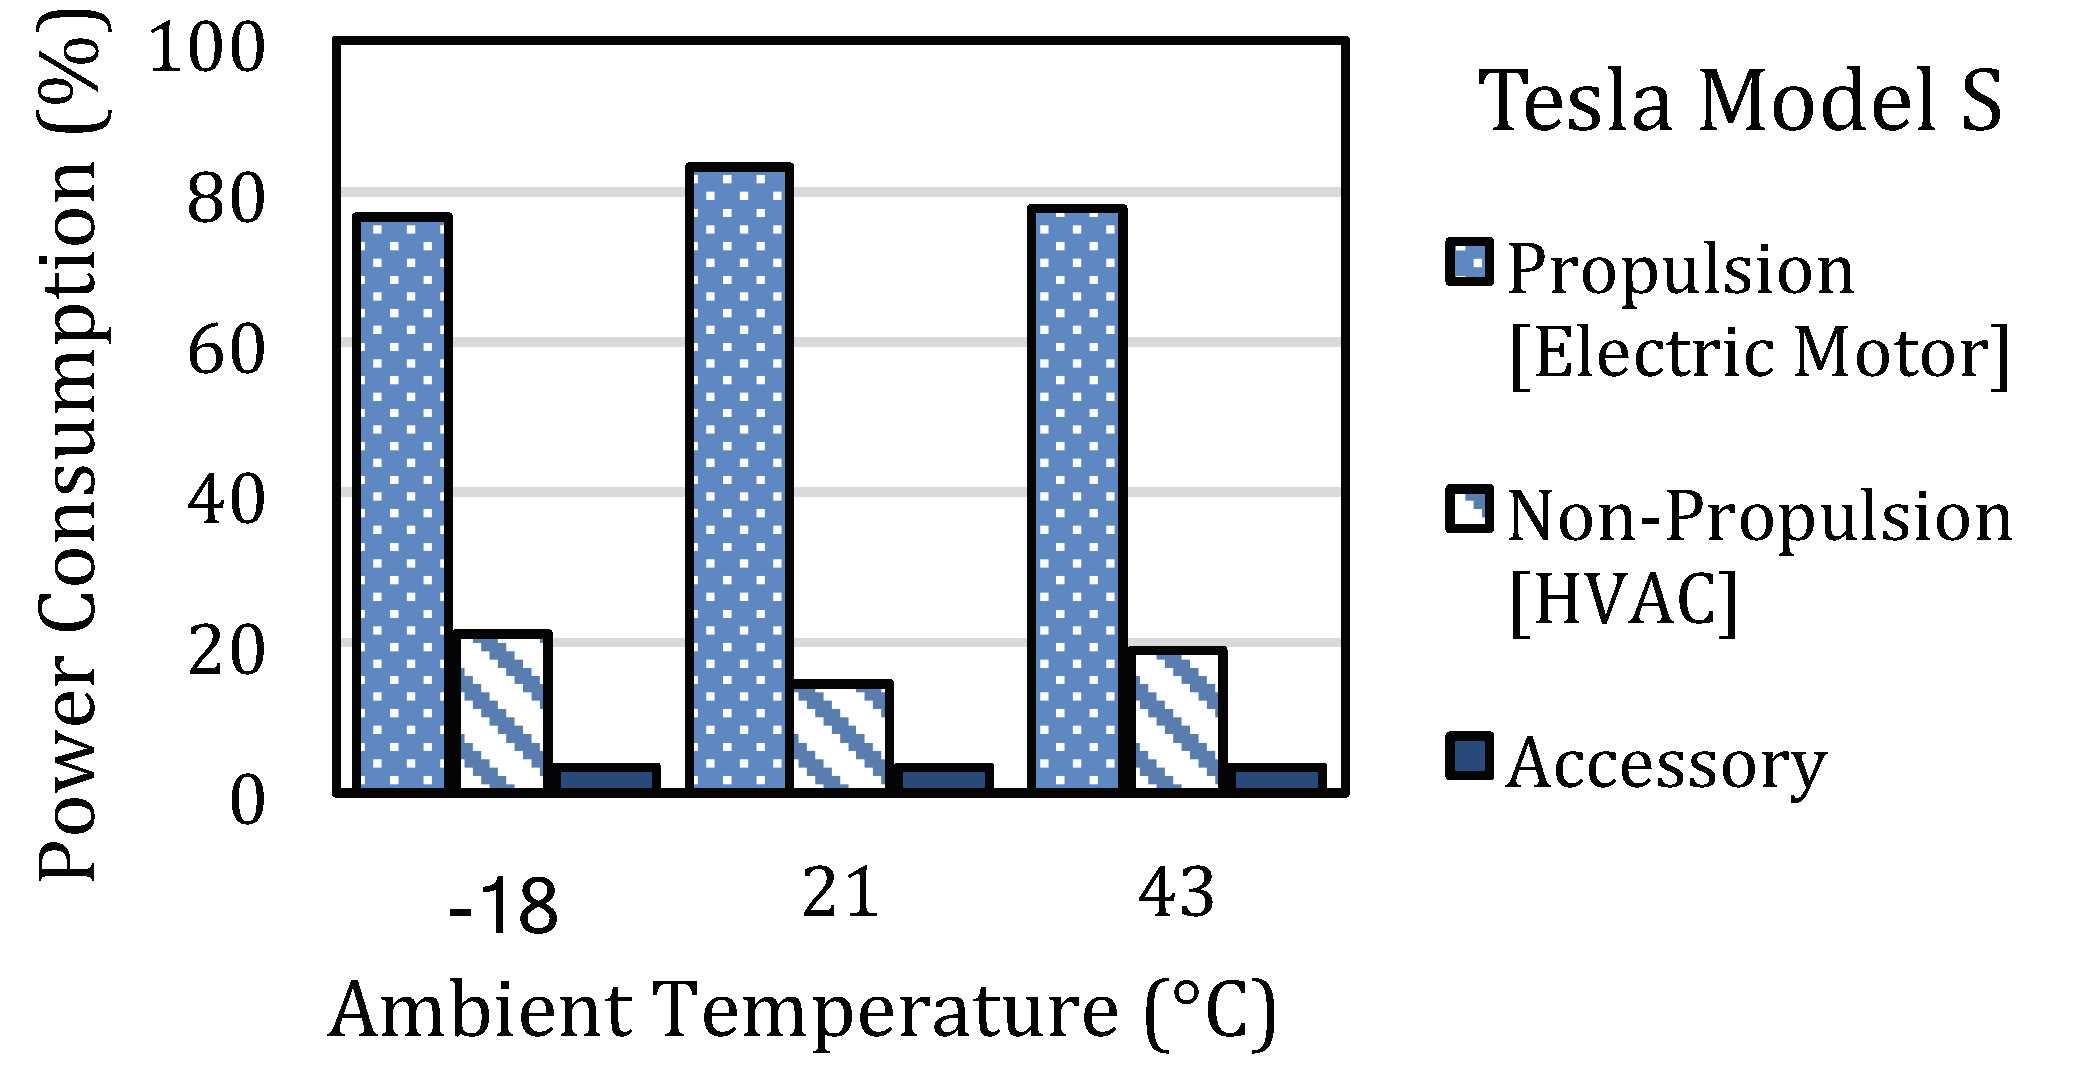
\includegraphics[width=0.7\hsize]{Figures/Al_Faruque/AF_figure2.jpeg}
\caption{Percentages of three types of power consumption in EV for different ambient temperatures~\cite{AF_1,AF_10}.}
\label{AF_image2}
\end{figure}      

Fig.~\ref{AF_image2} illustrates the details of different types of power consumption in a Tesla Model S EV. As shown in the figure, the fraction of the HVAC power consumption (non-propulsion) is mainly dependent on the ambient temperature and the required comfort range, not the driving profile (as opposed to the electric motor.) This characteristic shows that auxiliary systems have flexible load and power pattern. Hence, modeling and estimation of the auxiliary systems such as HVAC will enable the EV designers and engineers to further exploit this characteristic. Therefore, they will be able to adjust and optimize the non-propulsion power, e.g. HVAC power, in order to improve the operating parameters of the EV such as driving range and battery lifetime.

We will further discuss the details of modeling and estimation of the driving profile and non-propulsion power in the EV. Later, we will go further into the details of how the designers are able to optimize these variables at run time to improve the operating behavior of the EV.

%%%%%%%%%%%%%%%%%%%%%%%%%%%%%%%%
\subsection{Modeling and Estimation}

\subsubsection{Driving Profile}

Electric motor in EVs is the main system contributing to the total power consumption and generation. One of the main factors deciding this propulsion power request, is the driving behavior. The driving behavior is modeled by the values of the driving speed, acceleration, and deceleration at each time instance of the driving route. This model that is called \textbf{driving profile} depends on various parameters of driving such as route conditions and the driver characteristics~\cite{AF_1,AF_17}.

The driving profile can be generated based on the data gathered from one driver while driving, in order to model the \textit{\textbf{driver-specific}} driving profile; this can be achieved by monitoring multiple state variables of the EV at run time using On Board Diagnosis (OBD) device~\cite{AF_18}. For instance, a biometric system can be incorporated into vehicle security in order to identify the driver. In other words, the amount of pressure a driver applies on the accelerator and brake pedals have been utilized in modeling their driving behavior and personal identification~\cite{AF_19,AF_20}. Moreover, the anger and emotional aggressiveness of the driver may influence its driving behavior~\cite{AF_21,AF_22,AF_23}. Hence, researchers attempt to model these factors that define the driving profile so that they can analyze their influence. Moreover, the safety and energy consumption of the vehicle are important factors which are influenced by the driving behavior that need to be predicted~\cite{AF_23,AF_24}. 

On the other hand, the driving profile can also be generated based on the gathered data from all the drivers driving on a specific route, in order to model \textit{\textbf{route-specific}} driving profile. Certain navigation system databases like Google Maps~\cite{AF_25} generate these models as part of the traffic information of their map databases by gathering data from all their clients or the sensors implemented in the city roads. Moreover, the data of this generic driving behavior can be used to generate driving test cycles. The automotive manufacturers may use these driving cycles to test and analyze the performance of their vehicles in terms of energy consumption and emissions~\cite{AF_26,AF_27}.

In summary, these driving profile models can be used for the purpose of personal identification, driver characteristics estimation, or estimation of the propulsion power by the electric motor. Later on, they can be adjusted and optimized for a specific driver or driving route in order to improve the EV operation in terms of battery lifetime, driving range, or even safety.

Typically, driving profile can be implemented simply as a matrix of segments ($\bar{s}$)~\eqref{AF_eq1}. Each row of this matrix contains the time duration, length, average speed, average acceleration, and road slope of each segment of in the driving route. Each segment represents a portion of the route with different route condition and the corresponding driver reaction.

\begin{equation}
%\[
\bar{s} = 
\begin{bmatrix} 	
time 		& length 	& speed 	& acceleration 	& slope \\ 
t_1		&l_1		&v_1		&a_1			&\alpha_1	\\
\vdots 	&\vdots 	&\vdots 	&\vdots 		&\vdots \\
t_n		&l_n		&v_n		&a_n			&\alpha_n	
\end{bmatrix}
\label{AF_eq1}
%\]
\end{equation}

The values for these elements can be retrieved based on the data gathered for the drivers~\cite{AF_1,AF_11}.

\subsubsection{Non-Propulsion Power}

The amount of non-propulsion power requested in EV depends on the targeted auxiliary systems, their functioning components and the control process implemented to integrate and manage them.
For instance, an HVAC system is controlled by an automotive climate control in order to maintain the cabin temperature ($T_z$). The cabin temperature is influenced by the supply air ($T_s$) to the cabin and other thermal loads including the heat exchange with outside and the solar radiation. The air supply temperature is controlled by adjusting the temperature set points on heating and cooling coils. Moreover, variable air valves are utilized in more complex HVAC system in order to maintain the required thermal comfort for the passengers even in multi-zone cabin. These systems utilize variable-speed fans and air ducts to provide the supply air to the zone(s).

Typically, the power consumption of the cooling ($P_c$) and heating coils ($P_h$) depends on the energy difference between their inlet and outlet air flows. Moreover, the power consumption of the variable-speed fans ($P_f$) is quadratically related to the air flow rate ($\dot{m}_z$). The thermodynamics of the cabin temperature considering all the control inputs and variables are modeled by energy balance differential equations. Hence, Ordinary Differential Equations (ODE) can be implemented to model and estimate the thermodynamic behavior of the HVAC system and its the instantaneous power consumption. 

These models are typically used for evaluating and analyzing the performance of the auxiliary system – HVAC – and its influence on the whole vehicle. For instance, the researchers estimate the energy consumption of the HVAC system regarding different driving conditions like weather. This estimation is leveraged in order to predict the driving range of the vehicle and analyze how much HVAC influence this crucial parameter of the vehicle~\cite{AF_23,AF_28,AF_29}. 

%%%%%%%%%%%%%%%%%%%%%%%%%%%%%%%%
\subsection{Runtime Optimization}

During the operation of a CPS inside EVs, there are multiple control inputs which can be adjusted and optimized towards a certain objective. The controllers implemented are responsible to monitor the state variables and decide these control inputs. They may utilize the integrated modeling towards their estimation and optimization purpose. For instance, an Automotive Climate Control (ACC) senses the cabin temperature and weather and decides how hot and cool the supply air temperature should be given the model of the cabin~\cite{AF_30,AF_31,AF_32,AF_33}. Moreover, vehicles implement energy management methodologies is in order to improve the driving range by reducing the energy consumption.  For instance, the power split among the battery, combustion engine, and ultracapacitor is very important to the performance of the vehicle and its driving range. Predictive models are incorporated in the control to facilitate with the system estimation and control optimization~\cite{Park:DAC13,AF_10,AF_34,AF_35,AF_36}.

In the following, we explain the details of utilizing the two models of driving profile and non-propulsion power for system estimation and control optimization in their corresponding controllers.

\subsubsection{Driving Management}

Driving management and route optimization have always been the most common problem of vehicles to improve the quality of transportation. Typically, driving management methodologies consider the driving distance and the driving time in order to find the fastest and shortest route to a specific destination~\cite{AF_37,AF_38,AF_39}. Map databases are utilized to provide the required information for selecting the optimal route. More detailed driving profile modeling can enable the methodologies to optimize the driving routes considering other objectives such as energy consumption and the battery lifetime. For instance, driving profile model containing the segment information such as road slope and average speed will enable the driving management methodology to estimate the energy consumption of the electric motor at each segment. The routing algorithm can be implemented such that the edge weights of the graph are defined as same as the objective considered in the driving management~\cite{AF_40,AF_41,AF_42}. 

\begin{figure}
\centering
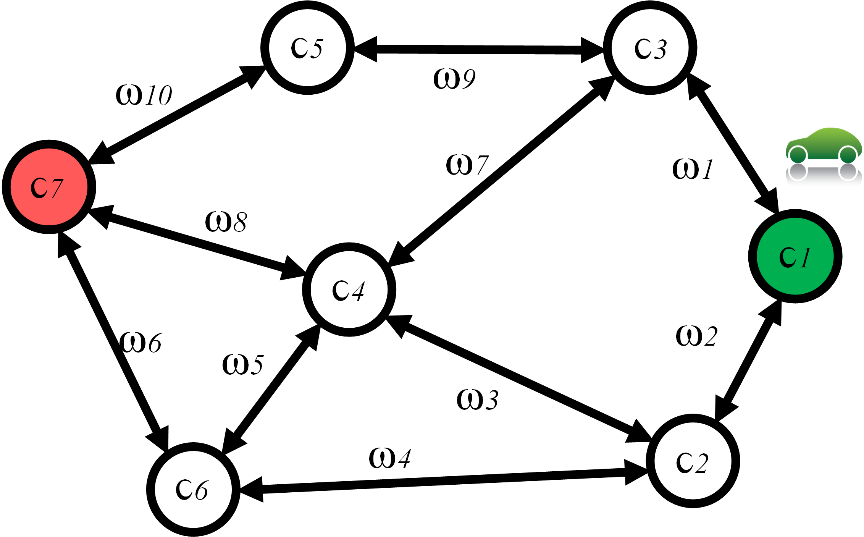
\includegraphics[width=0.7\hsize]{Figures/Al_Faruque/AF_figure3.png}
\caption{Routing problem labeled with edge weights~\cite{AF_11}.}
\label{AF_image3}
\end{figure}      

The results have shown that by sacrificing about 3 minutes of the driving time, a driving management can take a detailed driving profile modeling into account and reduce the energy consumption by 11.9\% compared to the fastest route~\cite{AF_11,AF_17}.

\subsubsection{Control Scheduling}

Auxiliary systems in EV implement control algorithms which are responsible for scheduling control actions in the systems. The decisions made by the controller will influence the non-propulsion power requested by the auxiliary systems.

For instance, as we stated before automotive climate control adjusts the control inputs into the HVAC system to maintain the cabin temperature around a certain target and within a comfort range. The climate control may be implemented using rule-based control or a MPC. The controller may leverage the HVAC system dynamic and non-propulsion power models to estimate the state, auxiliary, and output variables according to specific control inputs for a certain prediction horizon in the future. The controller utilizes an optimizer to adjust the control inputs such as heating and cooling coil temperature set points and the fan speed of the prediction horizon while considering the constraints. The controller may be responsible to minimize an objective or cost function. An ACC may only consider the cabin temperature as the objective~\cite{AF_30,AF_31,AF_32,AF_33}. The power consumption of the HVAC system may be considered as well in order to reduce the influence on the EV energy consumption and battery capacity loss~\cite{AF_10,AF_29}. Therefore, depending on the details of the modeling, the cost function may include the 1) cabin temperature variation, 2) non-propulsion (HVAC) energy consumption, and 3) battery capacity loss. Moreover, there are certain constraints on the control inputs and state variables which should be satisfied during the optimization and control process.

Therefore, the control scheduling of the auxiliary systems may reduce the battery stress, improve the driving range, and the battery lifetime by adjusting the non-propulsion power such that it compensates for the propulsion power or the quality of the system. It has been shown that MPC-based methodology is able to minimize the non-propulsion power on average 39\% compared to the fuzzy-based methodology which minimizes by 6\%~\cite{AF_10,AF_32,AF_43}.


